\tikzstyle{txt} = [text centered, inner sep=0pt]

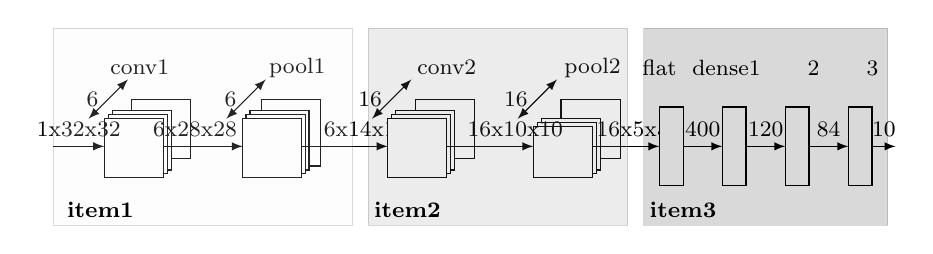
\begin{tikzpicture}[scale=1.0,
z={({0.3cm*cos(45)},{0.3cm*sin(45)})},
>=latex, 
font=\footnotesize,
]

% Big Input images



%CONV1
\draw[fill=white] (0.25+7*0.05-.6,7*0.05) rectangle (1+7*0.05-.6,.75+7*0.05);
\foreach \foreach \z in {2,...,0}  {%
 \draw[fill=white] (0.25+\z*0.05-.6,.1+\z*0.05) rectangle (1+\z*0.05-.6,.85+\z*0.05);
}
\draw (0.7-.6,1.5)node[txt] (conv1){conv1};
\draw[->] (-1,0.5) -- node[above] {$1$x$32$x$32$} (0.25-.6,0.5);
\draw[<->] (.25-0.2-.6,.85+0*0.05) -- node[left] {$6$} (.25+0.3-.6,.85+0.5);

%MAXPOOL1
\draw[fill=white] (2.5+5*0.05-1.1,5*0.05) rectangle (3.25+5*0.05-1.1,0.85+5*0.05);
\foreach \foreach \z in {2,...,0}  {%
 \draw[fill=white] (2.5+\z*0.05-1.1,0.1+\z*0.05) rectangle (3.25+\z*0.05-1.1,.85+\z*0.05);
}
\draw (3.2-1.1,1.5)node[txt] (conv1){pool1};
\draw[->] (1-.6,0.5) --(1.75-1.1,0.5) |- node[above,pos=0.6] {$6$x$28$x$28$} (2.51-1.1,0.5);
\draw[<->] (2.5-0.2-1.1,0.85+0*0.05) -- node[left] {$6$} (2.5+0.3-1.1,0.85+0.5);

%CONV2
\draw[fill=white] (4.75+7*0.05-1.5,7*0.05) rectangle (5.5+7*0.05-1.5,0.75+7*0.05);
\draw (5.5-1.5,1.5)node[txt] (conv1){conv2};
\draw[->] (3.25-1.1,0.5) -- (4-1.1,0.5) |- node[above,pos=0.6] {$6$x$14$x$14$} (4.75-1.5,0.5);
\foreach \foreach \z in {2,...,0}  {%
 \draw[fill=white] (4.75+\z*0.05-1.5,0.1+\z*0.05) rectangle (5.5+\z*0.05-1.5,0.85+\z*0.05);
}
\draw[<->] (4.75-0.2-1.5,0.85+0*0.05) -- node[left] {$16$} (4.75+0.3-1.5,0.85+0.5);

%MAXPOOL2
\draw[fill=white] (7+7*0.05-1.9,7*0.05) rectangle (7.75+7*0.05-1.9,0.75+7*0.05);
\foreach \foreach \z in {2,...,0}  {%
 \draw[fill=white] (7+\z*0.05-1.9,0.1+\z*0.05) rectangle (7.75+\z*0.05-1.9,0.75+\z*0.05);
}
\draw (7.75-1.9,1.5)node[txt] (conv1){pool2};
\draw[<->] (7-0.2-1.9,0.85+0*0.05) -- node[left] {$16$} (7+0.3-1.9,0.85+0.5);
\draw[->] (5.5-1.5,0.5) -- (6.25-1.5,0.5) |- node[above,pos=0.67] {$16$x$10$x$10$} (7-1.9,0.5);

\draw[->] (7.75-1.9,0.5) -- node[above,pos=0.6] {$16$x$5$x$5$} (9-2.3,0.5);

\draw[fill=white] (9-2.3,0) rectangle (9.3-2.3,1);
\draw[->] (9.3-2.3,0.5) -- node[above] {$400$} (9.8-2.3,0.5);
\draw (9-2.3,1.5)node[txt] (conv1){flat};

%dense1
\draw[fill=white] (9.8-2.3,0) rectangle (10.1-2.3,1);
%dense2
\draw[fill=white] (10.6-2.3,0) rectangle (10.9-2.3,1);
%dense3
\draw[fill=white] (11.4-2.3,0) rectangle (11.7-2.3,1);
\draw[->] (10.1-2.3,0.5) --node[above] {$120$}(10.6-2.3,0.5);
\draw[->] (10.9-2.3,0.5) --node[above] {$84$} (11.4-2.3,0.5);
\draw (10.5-2.2,1.5)node[txt] (conv1){dense1 \hspace{.4cm} 2 \hspace{.4cm} 3};



\draw[->] (11.7-2.3,0.5) -- node[above] {$10$} (12-2.3,0.5);


\coordinate (item1A) at (-1 , -.5);
\coordinate (item1B) at (2.8, 2);       
\draw [fill=gray!10, opacity=.15](item1A) rectangle (item1B) 
                    node[xshift=-3.2cm, yshift=-2.3cm, opacity=1] {\textbf{item1}};

\coordinate (item2A) at (3 , -.5); 
\coordinate (item2B) at (6.3 , 2); 
 \draw [fill=gray!100, opacity=.15](item2A) rectangle (item2B) 
                    node[xshift=-2.8cm, yshift=-2.3cm, opacity=1] {\textbf{item2}};


\coordinate (item3A) at (6.5 , -.5);
\coordinate (item3B) at (9.6 , 2); 
 \draw [fill=gray!200, opacity=.15](item3A) rectangle (item3B) 
                    node[xshift=-2.6cm, yshift=-2.3cm, opacity=1] {\textbf{item3}};
\end{tikzpicture}
